%%%%%%%%%%%%%%%%%%%%%%%%%%%%%%%%%%%%%%%%% % a0poster Landscape Poster % LaTeX Template % Version 1.0 (22/06/13) % % The a0poster class was created by: % Gerlinde Kettl and Matthias Weiser (tex@kettl.de) % % This template has been downloaded from: % http://www.LaTeXTemplates.com % % License: % CC BY-NC-SA 3.0 (http://creativecommons.org/licenses/by-nc-sa/3.0/)
%
%%%%%%%%%%%%%%%%%%%%%%%%%%%%%%%%%%%%%%%%%

%----------------------------------------------------------------------------------------
%	PACKAGES AND OTHER DOCUMENT CONFIGURATIONS
%----------------------------------------------------------------------------------------

\documentclass[a0,landscape]{a0poster}

\usepackage{multicol} % This is so we can have multiple columns of text side-by-side
\columnsep=100pt % This is the amount of white space between the columns in the poster
\columnseprule=3pt % This is the thickness of the black line between the columns in the poster

\usepackage[svgnames]{xcolor} % Specify colors by their 'svgnames', for a full list of all colors available see here: http://www.latextemplates.com/svgnames-colors

%\usepackage{times} % Use the times font
\usepackage{palatino} % Uncomment to use the Palatino font
%\usepackage{ClearSans}

\usepackage{graphicx} % Required for including images
\graphicspath{{figures/}} % Location of the graphics files
\usepackage{booktabs} % Top and bottom rules for table
\usepackage[font=small,labelfont=bf]{caption} % Required for specifying captions to tables and figures
\usepackage{amsfonts, amsmath, amsthm, amssymb} % For math fonts, symbols and environments
\usepackage{wrapfig} % Allows wrapping text around tables and figures
\usepackage{tcolorbox}
\usepackage{subfig}
%\usepackage[margin={5cm,2.5cm}]{geometry}
\usepackage{bm}
\usepackage[parfill]{parskip}

%\newcommand{\gw}{gravitational wave }
%\newcommand{\gws}{gravitational waves }
\newcommand{\subgw}{_{\textrm{\scriptsize{GW}}}}
\newcommand{\ee}[1]{\!\times\!10^{#1}}
\newcommand{\prob}{{\rm Pr}}
\newcommand{\grbrate}{{{\mathcal R}_{\mathrm{grb}}}}
\newcommand{\cbcrate}{{{\mathcal R}}}
\newcommand{\diff}{{\mathrm d}}
\newcommand{\rhostar}{{\rho^*}}

\newcommand{\matr}[1]{\mathbf{#1}}
\newcommand{\tran}[1]{#1^{\top}}

\DeclareMathOperator*{\argmin}{arg\,min}
\DeclareMathOperator*{\argmax}{arg\,max}

\def\imbh#1{intermediate mass black hole#1(IMBH#1)\gdef\imbh{IMBH}}
\def\smbh#1{supermassive black hole#1(SMBH#1)\gdef\smbh{SMBH}}
\def\bbh#1{binary black hole#1 (BBH#1)\gdef\bbh{BBH}}
\def\bh#1{black hole#1 (BH#1)\gdef\bh{BH}}
\def\ns#1{neutron star#1 (NS#1)\gdef\ns{NS}}
\def\gw#1{gravitational wave#1 (GW#1)\gdef\gw{GW}}
\def\sn#1{core-collapse supernova#1 (CCSN#1)\gdef\sn{CCSN}}
\def\pnw#1{post-Newtonian#1 (PN#1)\gdef\pnw{PN}}
\def\eos#1{equation of state#1 (EOS#1)\gdef\eos{EOS}}
\def\grb#1{gamma-ray burst#1 (GRB#1)\gdef\grb{GRB}}
\def\amr#1{adaptive mesh refinement#1 (AMR#1)\gdef\amr{AMR}}
\def\isco#1{innermost stable circular orbit#1 (ISCO#1)\gdef\isco{ISCO}}
\def\cwb#1{Coherent WaveBurst#1 (CWB#1)\gdef\cwb{CWB}}

\def\prd{Phys. Rev. D.}

\begin{document}

%----------------------------------------------------------------------------------------
%	POSTER HEADER 
%----------------------------------------------------------------------------------------

% The header is divided into three boxes:
% The first is 55% wide and houses the title, subtitle, names and university/organization
% The second is 25% wide and houses contact information
% The third is 19% wide and houses a logo for your university/organization or a photo of you
% The widths of these boxes can be easily edited to accommodate your content as you see fit

\begin{minipage}[b]{0.73\linewidth}
\veryHuge \color{NavyBlue} \textbf{Binary Neutron Star Gravitational Wave
Bursts:  \\A Post-Merger Model Using Principal Component Analysis} \color{Black}\\ \\% Title
\huge \textbf{James A. Clark$^{1}$, Andreas Bauswein$^{2}$ \& Nikolaos Stergioulas$^{2}$}\\ \\% Author(s)
\large 1. Georgia Institude of Technology\\ % University/organization
\large 2. Aristotle University of Thessaloniki\\ % University/organization
\end{minipage}
%
\hspace{2.5cm}
%
\begin{minipage}[b]{0.25\linewidth}
    
\includegraphics[height=5cm]{cra.png} \hspace{1cm}

\includegraphics[height=5cm]{thessaloniki.png} % Logo or a photo of you, adjust its dimensions here
~\\~\\~\\~\\~\\~\\
\end{minipage}

\vspace{1cm} % A bit of extra whitespace between the header and poster content

%----------------------------------------------------------------------------------------

\begin{multicols}{4} % This is how many columns your poster will be broken into, a poster with many figures may benefit from less columns whereas a text-heavy poster benefits from more

%----------------------------------------------------------------------------------------
%	ABSTRACT
%----------------------------------------------------------------------------------------

    \begin{comment}
        \color{Navy} % Navy color for the abstract

        \begin{abstract}

            Sed fringilla tempus hendrerit. Vestibulum ante ipsum primis in faucibus orci
            luctus et ultrices posuere cubilia Curae; Etiam ut elit sit amet metus lobortis
            consequat sit amet in libero. Lorem ipsum dolor sit amet, consectetur adipiscing
            elit. Phasellus vel sem magna. Nunc at convallis urna. isus ante. Pellentesque
            condimentum dui. Etiam sagittis purus non tellus tempor volutpat. Donec et dui
            non massa tristique adipiscing. Quisque vestibulum eros eu. Phasellus imperdiet,
            tortor vitae congue bibendum, felis enim sagittis lorem, et volutpat ante orci
            sagittis mi. Morbi rutrum laoreet semper. Morbi accumsan enim nec tortor
            consectetur non commodo nisi sollicitudin. Proin sollicitudin. Pellentesque eget
            orci eros. Fusce ultricies, tellus et pellentesque fringilla, ante massa luctus
            libero, quis tristique purus urna nec nibh.

        \end{abstract}
    \end{comment}

%----------------------------------------------------------------------------------------
%	INTRODUCTION
%----------------------------------------------------------------------------------------
%\color{SaddleBrown} % SaddleBrown color for the introduction
\color{DarkSlateGray} % DarkSlateGray color for the rest of the content

%\section*{Introduction}


%----------------------------------------------------------------------------------------
%	OBJECTIVES
%----------------------------------------------------------------------------------------


%\begin{tcolorbox}[width=\columnwidth, colback={green}, title={Objective},
%    colbacktitle=yellow, coltitle=blue]
%    BLAH
%\end{tcolorbox} 

\color{DarkSlateGray} % DarkSlateGray color for the rest of the content

\section*{\centering Outline}

\begin{enumerate}
\item Binary neutron star mergers are likely to result in the formation of a
    stable / quasi-stable, differentially rotating neutron star
    remnant~\cite{shibata:06bns, giacomazzo:11, hotokezaka:11, bauswein:12}.
\item Transient non-axisymmetric deformations and $f$-mode oscillations
    $\rightarrow$ short (10--100\,ms) burst of high-frequency ($\sim $\,kHz)
    \gw{} emission.
\item Spectral properties of this burst carry finger prints of neutron star
    equation of state, particularly the dominant peak frequency $f_{\rm
    peak}$~\cite{hotokezaka:13,bauswein:14}.
\item May be observable to $\sim$10--50\,Mpc in advanced LIGO (c. 2020+), with a matched filter.
\item \emph{Merger \& post-merger phase are not well-modelled} \& unmodelled
    burst searches currently struggle to reconstruct the full time-frequency
    structure, which can be disjoint in the TF-plane.
\item We {\bf propose a method to construct a phenomelogical waveform model,
    based on principal component analysis of numerical merger simulations},
    to allow more {\bf robust identification and characterisation} of this
    high frequency component of the \gw{} signal from binary neutron star coalescence.
\end{enumerate}

%----------------------------------------------------------------------------------------
%	MATERIALS AND METHODS
%----------------------------------------------------------------------------------------

%\section*{\centering BNS \& High-frequency GW Bursts}
%
% Example Waveform: Shen 1.35+1.35
%\begin{center}%\vspace{1cm}
%    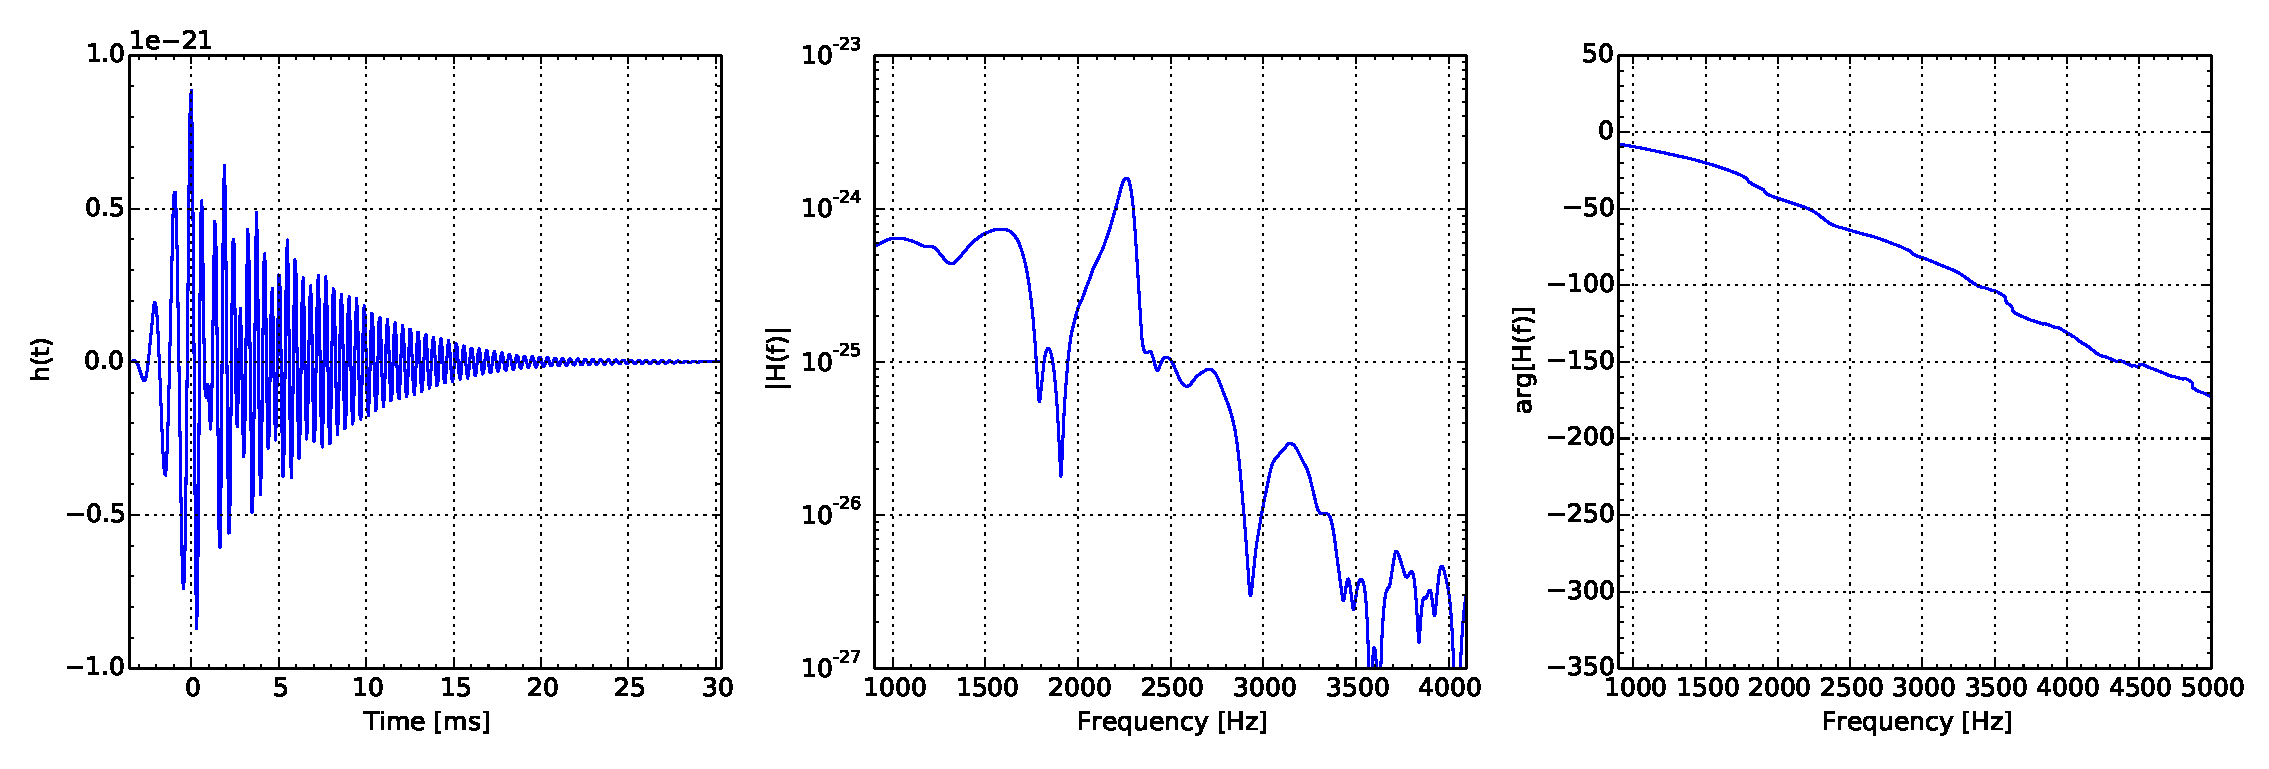
\includegraphics[width=\linewidth]{example_waveform.pdf}%
%    \captionof{figure}{\label{fig:example1} Example BNS-Burst Waveform}
%\end{center}%\vspace{1cm}
%
%
%   \begin{center}%\vspace{1cm}
%       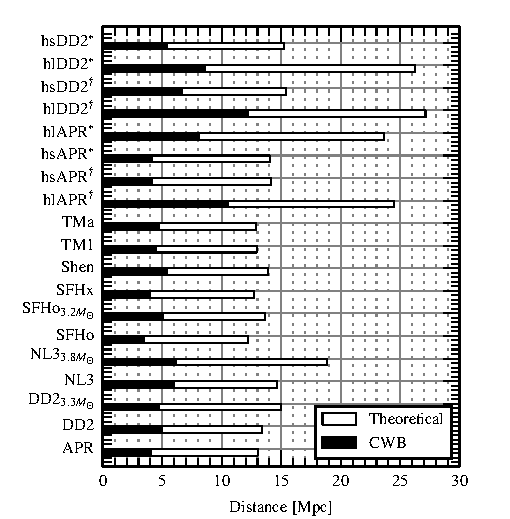
\includegraphics[width=0.5\linewidth]{distances.pdf}
%       \captionof{figure}{\label{fig:distances} Comparison of burst \& optimal
%   matched-filter Ranges, taken from the study reported
%   in~\cite{2014PhRvD..90f2004C}.}
%   \end{center}%\vspace{1cm}

%\vspace{-2.5cm}
\section*{\centering Principal Component Analysis \& Approximate Waveform Modelling}

{\bf \textsc{Objective}}: Given a collection of numerical waveforms, with no analytic
model, construct a \emph{reduced} set of basis functions from which we can
construct any one waveform to reasonable accuracy

\begin{enumerate}
    \item Organise $N$ waveforms, each containing $M$ samples, from
        numerical simulations of binary neutron star mergers into an $M\times N$
        data matrix, $\matr{X}$
    \item Align dominant features (see below), and center the data (subtract the
        mean waveform, $\matr{h}$) to get centered data matrix
        \begin{equation}
        \matr{Y}=\matr{X}-\matr{h}
    \end{equation}
    \item Find the eigenvectors $\matr{W}$ of the covariance matrix
        \begin{equation}
        \matr{C} = \tran{\matr{Y}}\matr{Y},
    \end{equation}
\item Using $\matr{W}$, we can find the principal component
        decomposition of $\matr{X}$,
        \begin{equation}\label{eq:pca}
            \matr{Z} = \matr{X} \matr{W},
        \end{equation}
        where $\matr{W}$ has been sorted in order of descending eigenvalues, and
        $\matr{Z}$ is the \emph{score matrix}, first $p<N$ columns of
        which represent our reduced basis\footnote{One takes care, of course, to
        add the mean waveform $\matr{h}$ back on to the waveform reconstructed
    from $\matr{Z}$}.
    \item Implemented via singular value decomposition, $\matr{X} =
        \matr{U}\matr{\Sigma}\tran{\matr{W}}$ so that,
        \begin{equation}
            \matr{Z} = \matr{X} \matr{W} =
            \matr{U}\matr{\Sigma}\matr{W}\tran{\matr{W}} = \matr{U}\matr{\Sigma}
        \end{equation}
\end{enumerate}


\vspace{9cm}
\subsection*{\centering Feature Alignment}
Goal is to use PCA to model \emph{variance} in data matrix $\matr{X}$
$\rightarrow$ important to align common features so that PCA picks out true
\emph{differences} in waveforms.

BNS merger waveforms exhibit varied broadband frequency content \& large
($\sim$\,kHz) differences between post-merger oscillations frequencies.  Natural
to work in the frequency domain with amplitude and phase spectra.

{\bf Key component to our analysis: align the magnitude (and phase) spectra} to
a common reference frequency, prior to PCA.   Alignment procedure:
\begin{enumerate}
    \item Construct spectrum of waveform, $H(f) = A(f)\exp[i\phi(f)]$
    \item Compute a new set of frequencies to scale $H(f)$ such that the
        dominant post-merger peak lies at $f_{\rm ref}$:
            $f_{\rm shift} = \frac{f_{\rm ref}}{f_{\rm peak}}  f$
    \item Interpolate the spectrum $H(f)\rightarrow H(f_{\rm shift})$ \& yield a
        new, shifted spectrum whose dominant post-merger oscillation frequency
        lies at $f_{\rm ref}$
    \item Perform PCA for magnitude \& phase spectra (separately)
    \item The original waveform can then be reconstructed by summation of
        the chosen principal component basis waveforms, followed by the inverse
        of the frequency shift operation to the desired $f_{\rm peak}$.
\end{enumerate}

%\vspace{-0.5cm}
\section*{\centering Waveform Catalogue \& Decomposition}
Here, we use the sample of numerical waveforms discussed
in~\cite{2014PhRvD..90f2004C},  which consists of {\bf ten waveforms with 8
equations of state}.  For the purposes of this study, the salient detail is that
these {\bf waveforms span the full space of frequencies, while sharing a
generally similar morphology}.  Figure~\ref{fig:catalogue} shows the spectra of
full catalogue overlaid with each other.  An example of a typical waveform in
the time domain can be found in figure~\ref{fig:example}.

%
% Catalogue F-domain
%
\begin{minipage}{\columnwidth}
\makeatletter
\newcommand{\@captype}{figure}
\makeatother
\centering
\subfloat[Magnitude Spectra]{%
  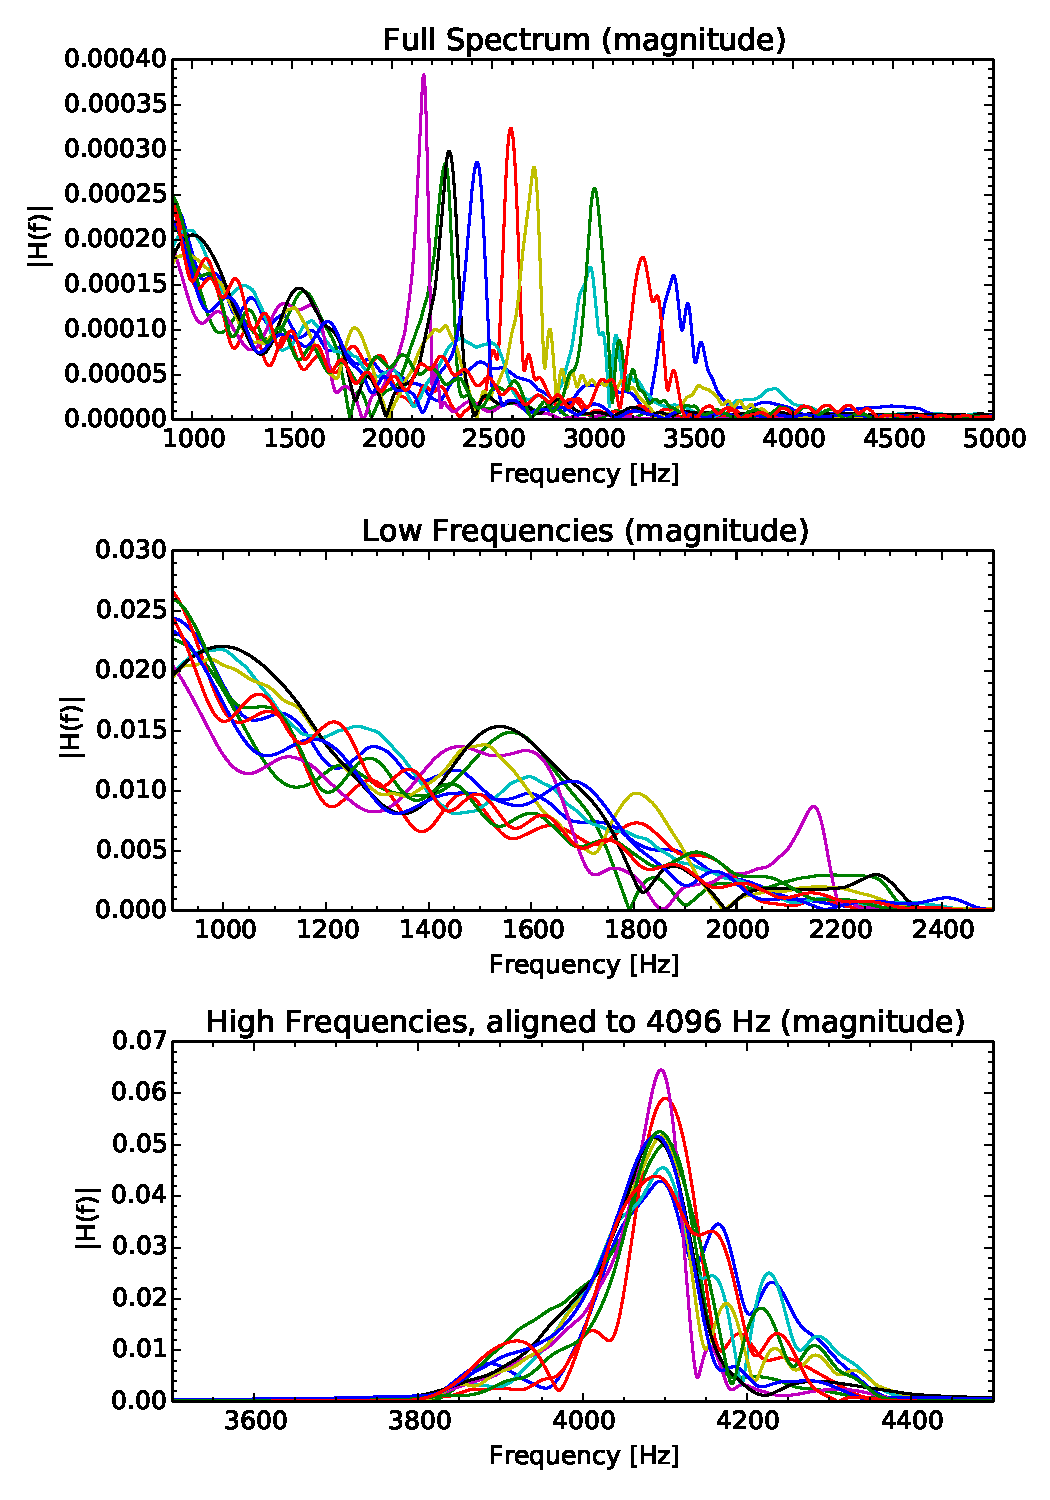
\includegraphics[width=0.45\linewidth]{catalogue_magnitude_overlay.pdf}%
  \label{fig:catalogue}%
}\qquad%
\subfloat[Principle Component Scores]{%
  %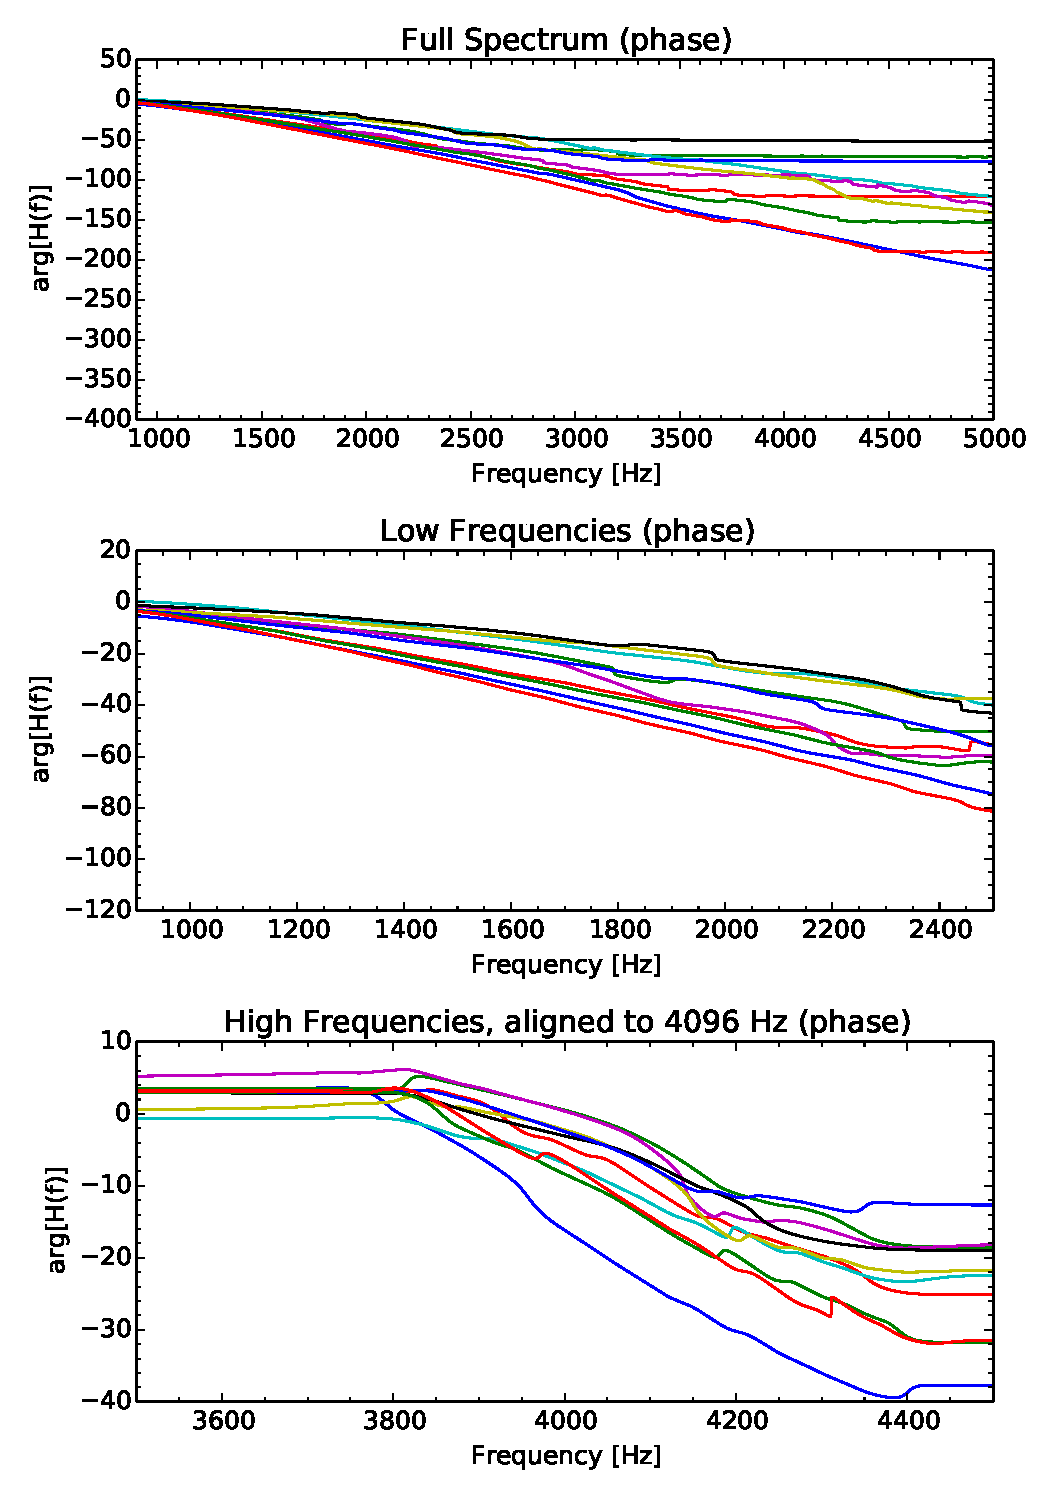
\includegraphics[width=0.45\linewidth]{catalogue_phase_overlay.pdf}%
  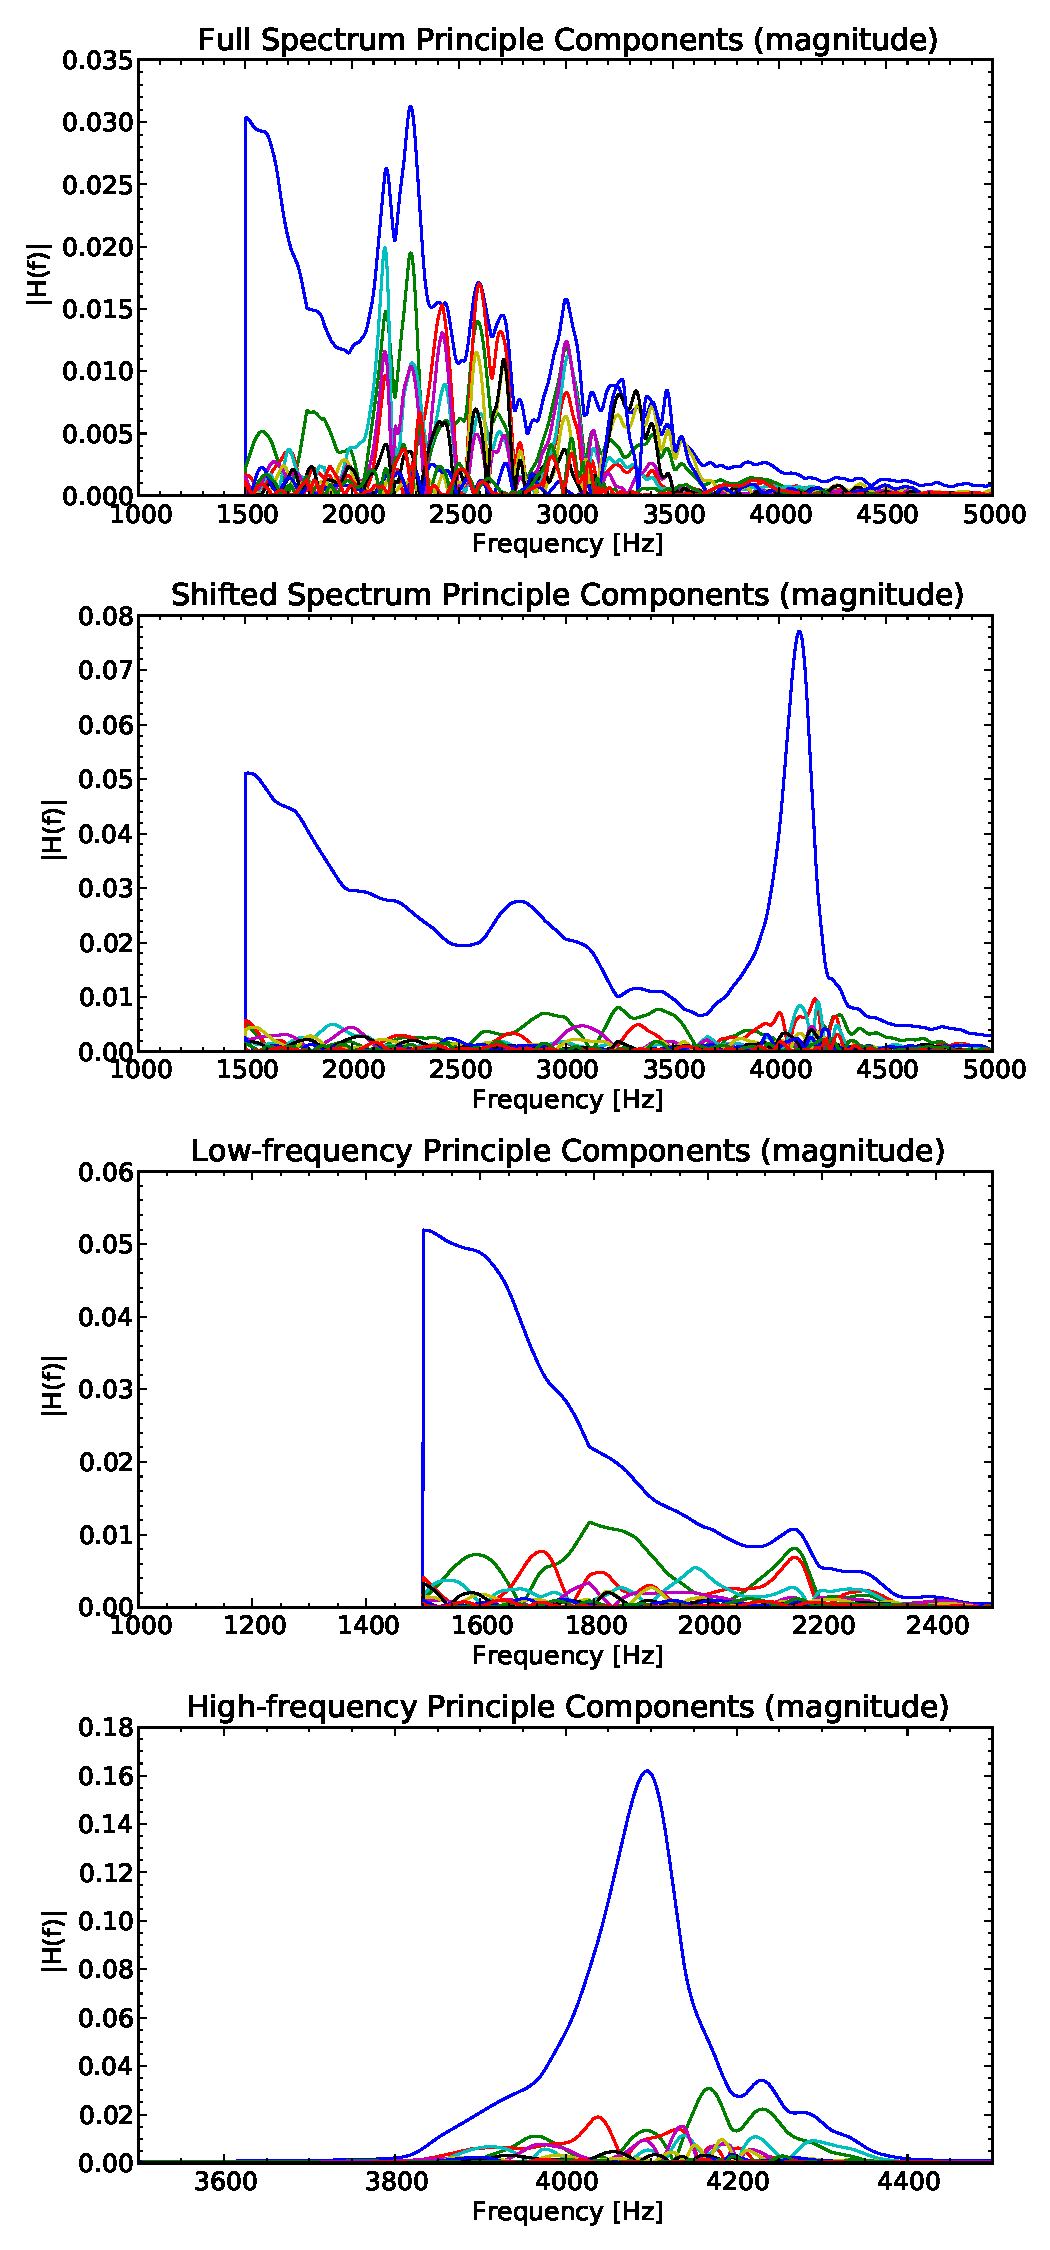
\includegraphics[width=0.45\linewidth]{pcs_magnitude_overlay.pdf}%
  \label{fig:}%
}
\caption{\emph{Top row}: magnitude spectra (left) and principal component
scores (right) of the original waveforms.  Note the wide range in peak
locations and variety of peak locations in the scores.  \emph{Bottom row}:
spectra following the frequency shifting procedure and the corresponding PC
scores.  Waveform frequencies have been scaled such that the peaks align at
1\,kHz (red vertical line).  Only a few scores now dominate.}
\end{minipage}

%   \subsection*{\centering Principal Component Basis, $\matr{Z}$}
%   %
%   % PCs F-domain
%   %
%   \begin{minipage}{\columnwidth}
%   \makeatletter
%   \newcommand{\@captype}{figure}
%   \makeatother
%   \centering
%   \subfloat[PC Magnitudes]{%
%     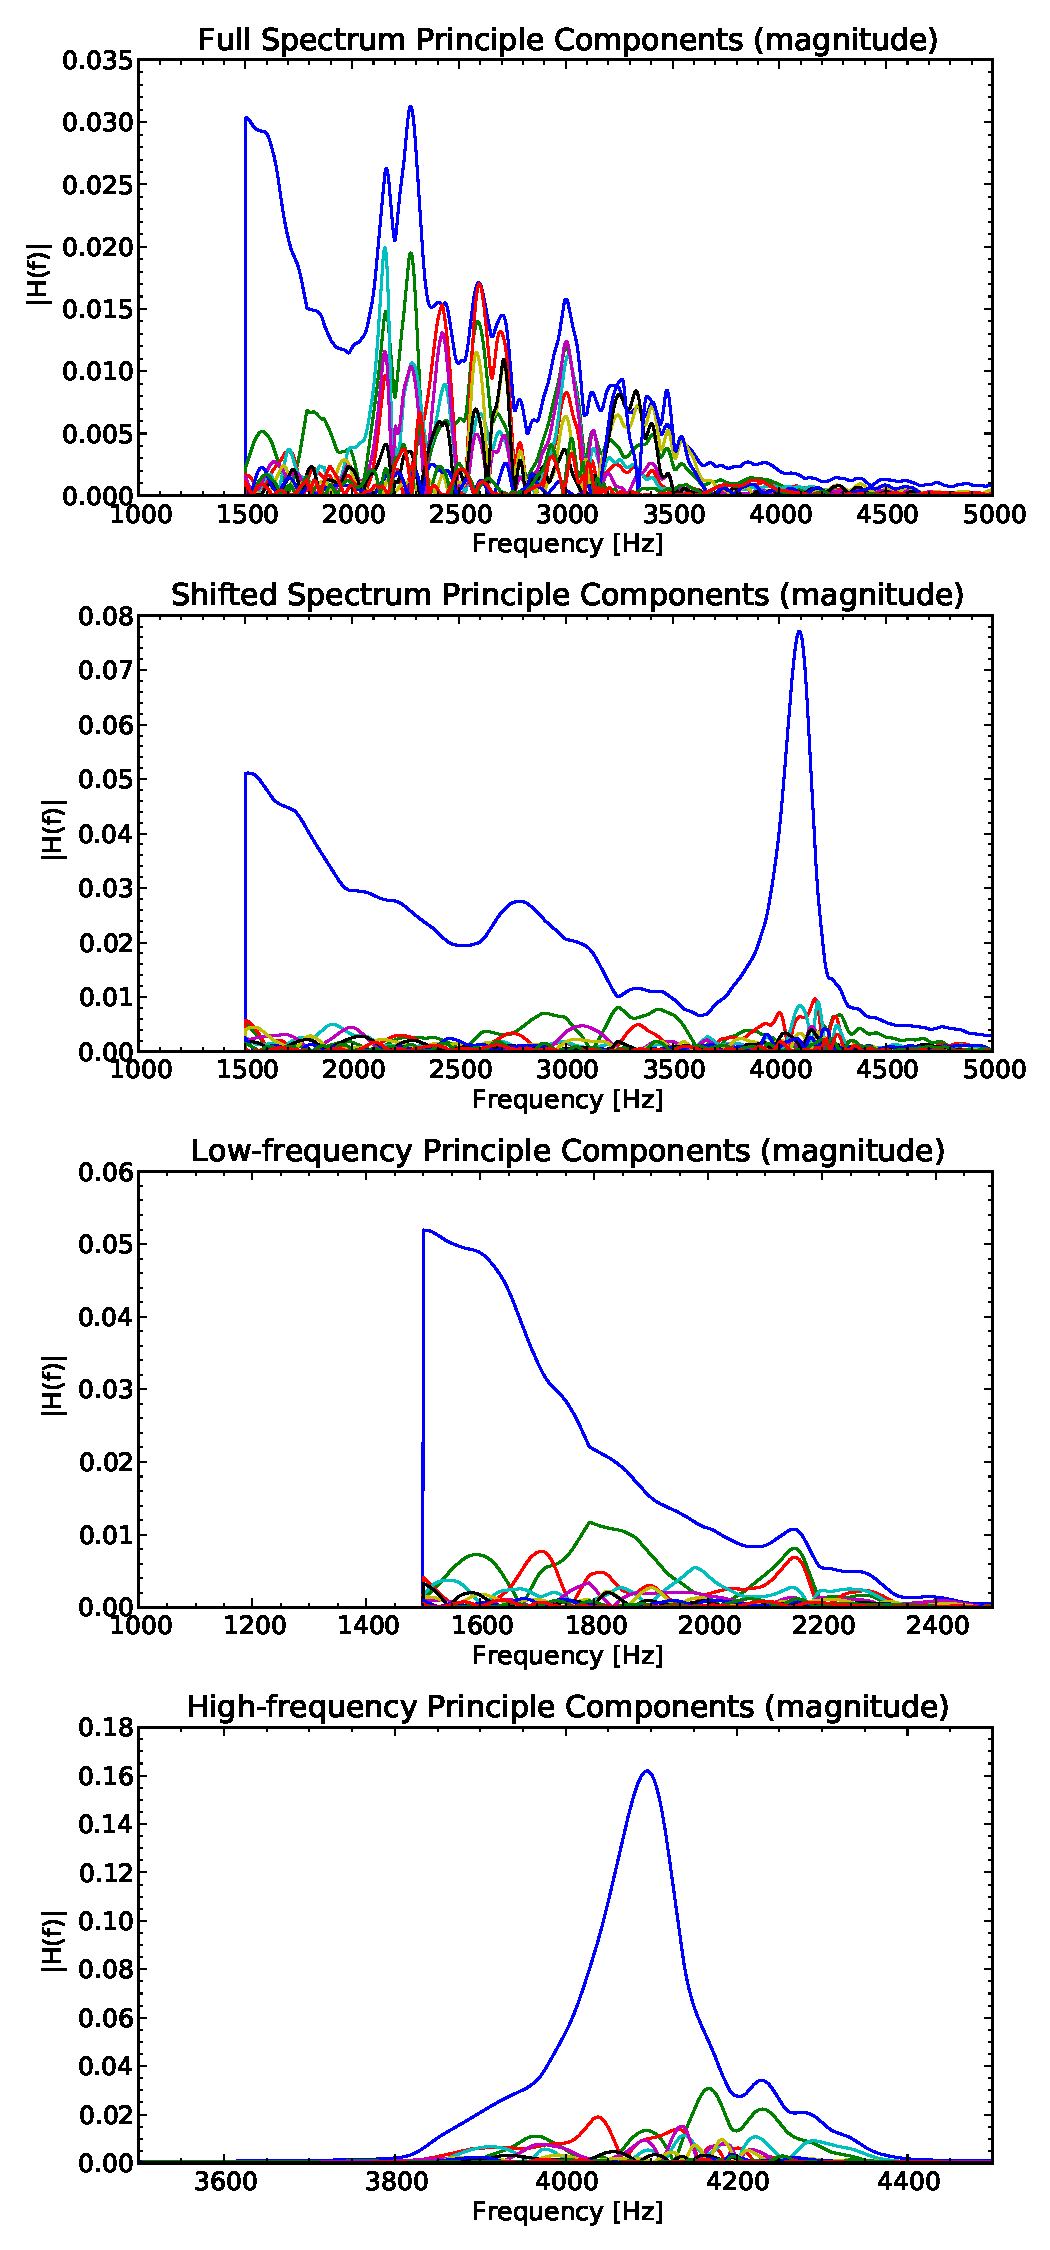
\includegraphics[width=0.45\linewidth]{pcs_magnitude_overlay.pdf}%
%     \label{fig:}%
%   }\qquad%
%   \subfloat[PC Phases]{%
%     %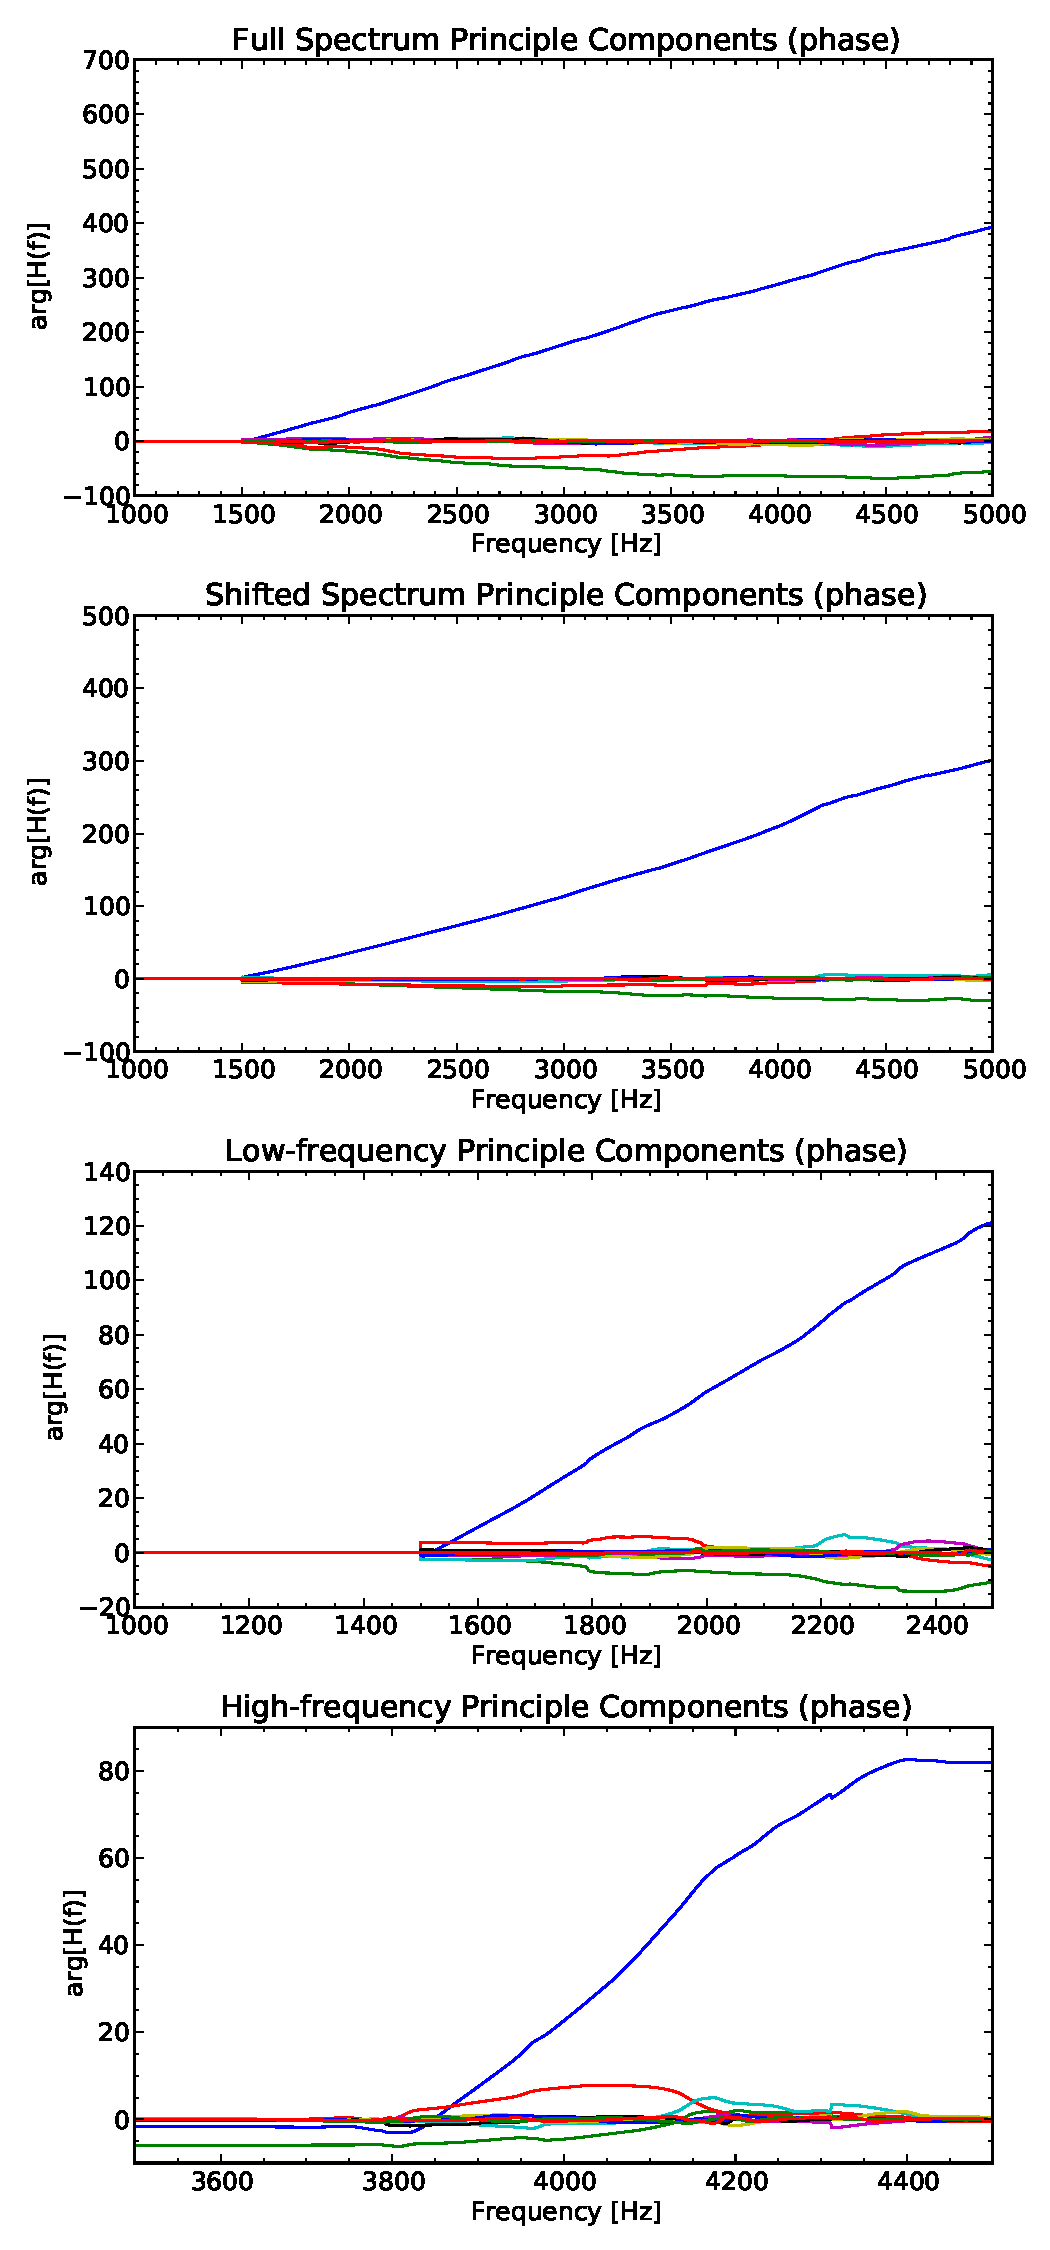
\includegraphics[width=0.45\linewidth]{pcs_phase_overlay.pdf}%
%     \label{fig:}%
%   }
%   \caption{Principal component scores for the magnitude (left) and phase (right)
%       spectra of our catalogue.  Note that the data matrices have been centered,
%       prior to the PCA; these figures demonstrate the dominant features in the
%       waveforms \emph{after mean subtraction}.  \emph{Top row}: principal
%       component scores for the original, unaligned data. \emph{Bottom row}:
%   principal component scores for the scaled and aligned spectra.}
%   \end{minipage}

\section*{\centering Demonstration}
\begin{minipage}{\columnwidth}
\makeatletter
\newcommand{\@captype}{figure}
\makeatother
\centering
\subfloat[First principal component]{%
  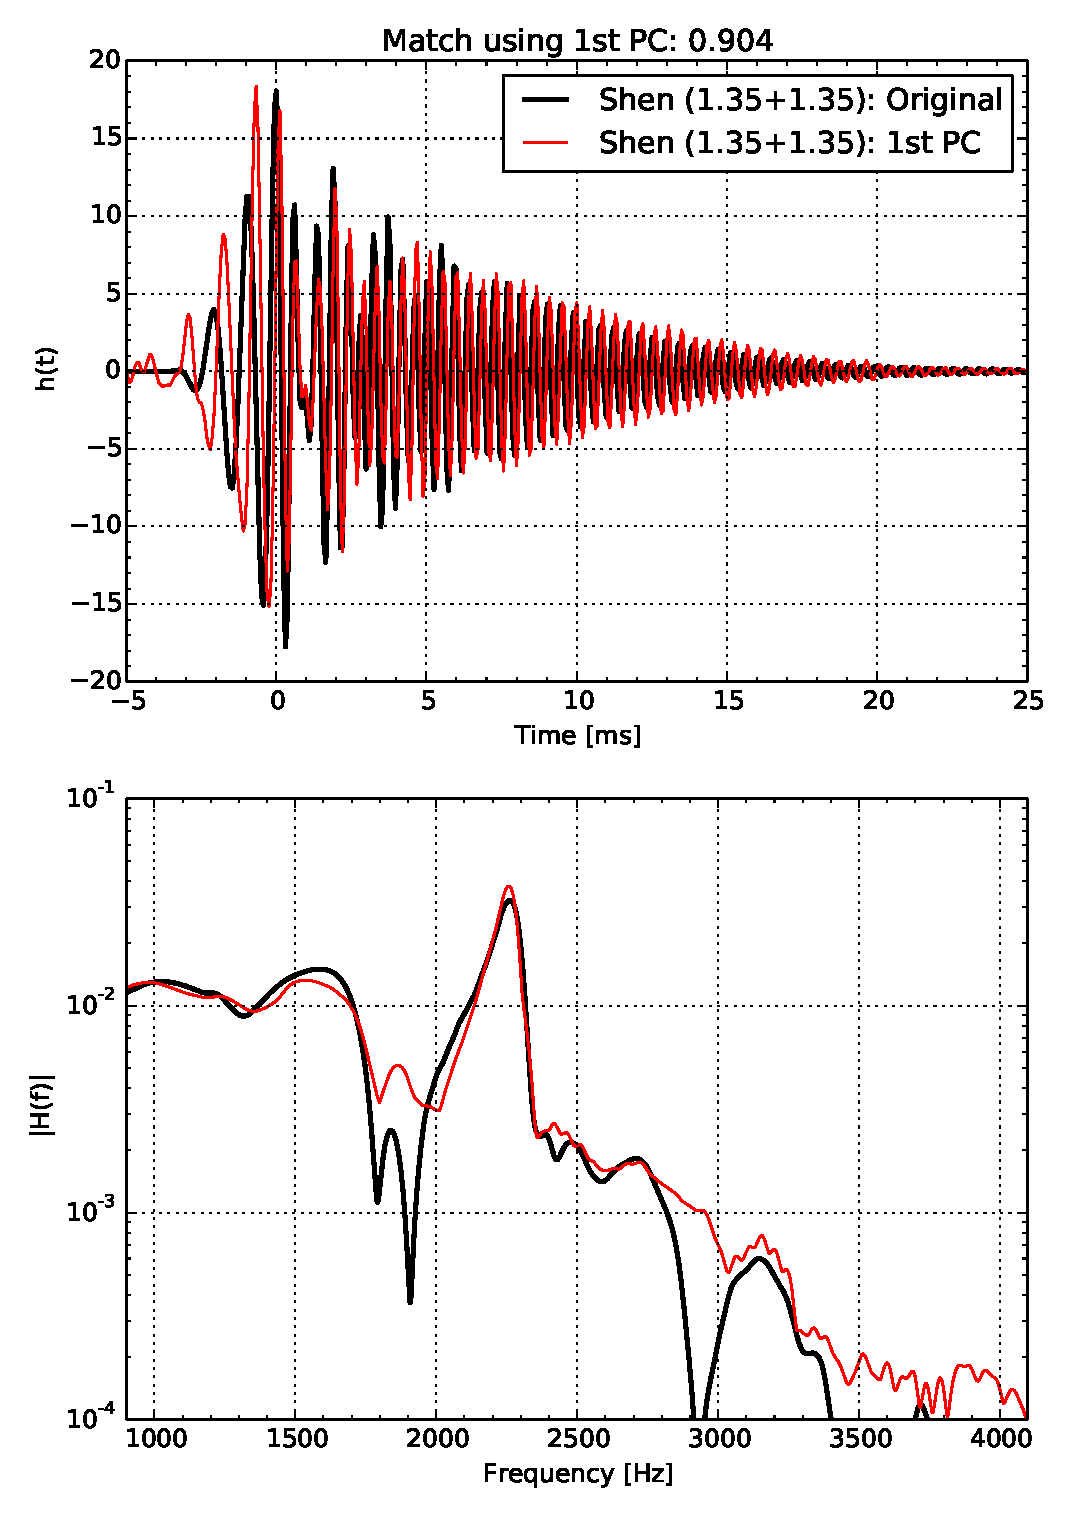
\includegraphics[width=0.4\linewidth]{firstPC_example_waveform_reconstruction.pdf}%
  \label{fig:}%
}\qquad%
\subfloat[All principal components]{%
  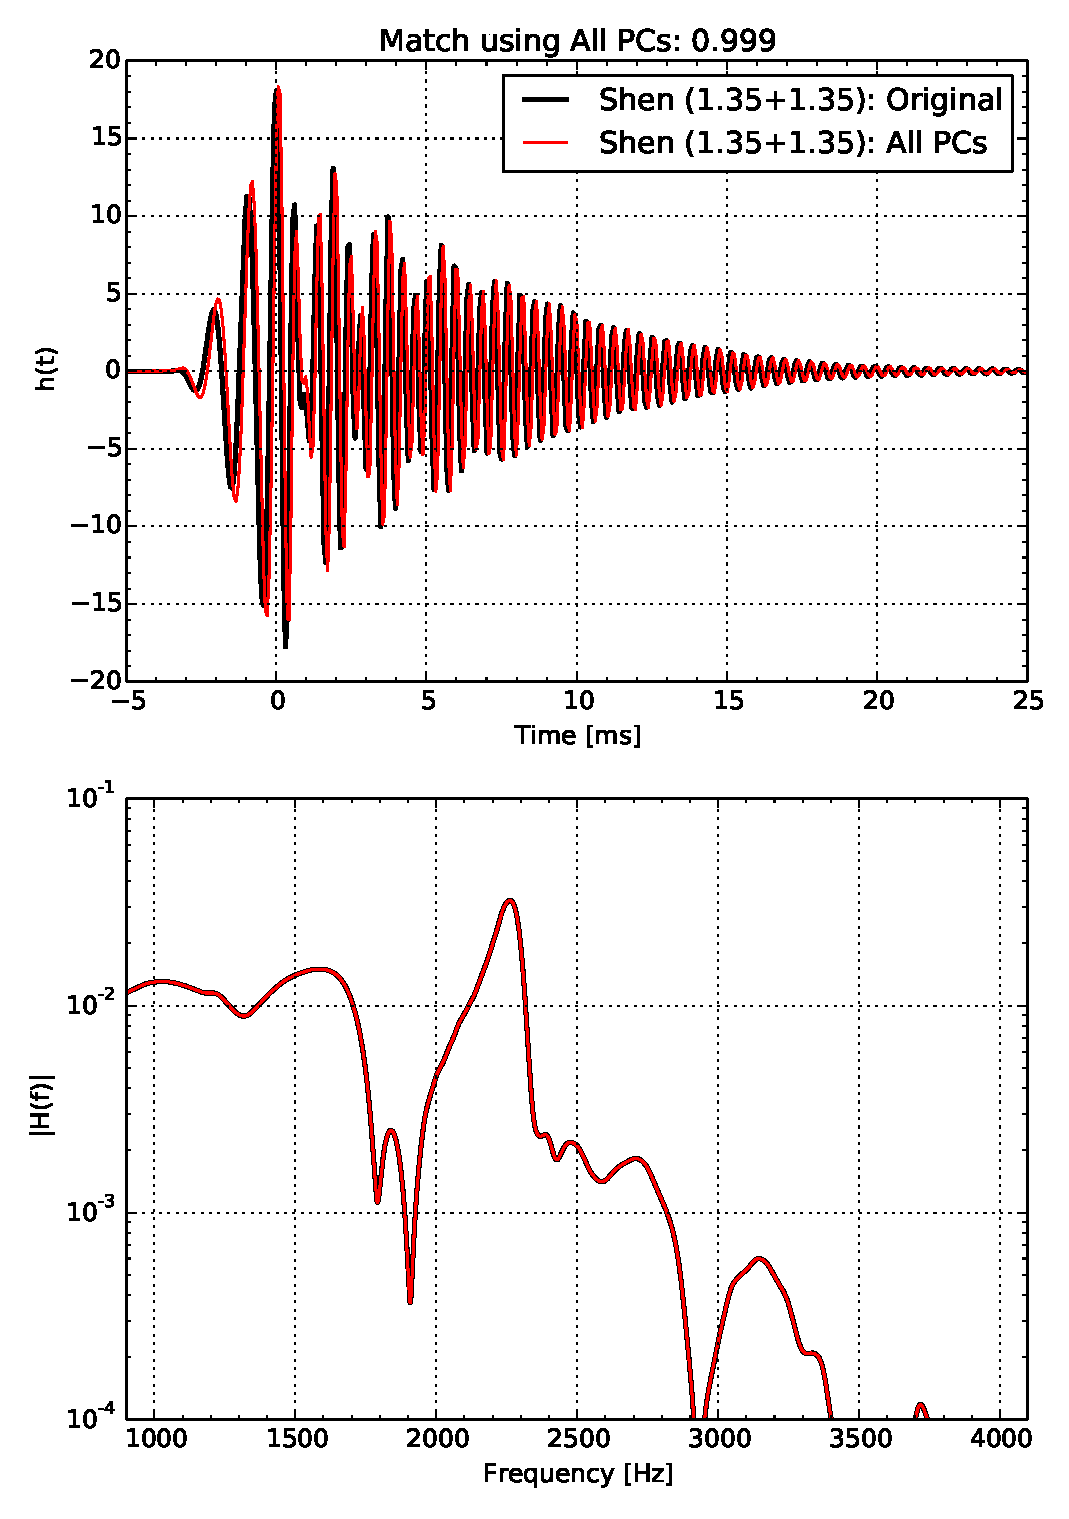
\includegraphics[width=0.4\linewidth]{allPCs_example_waveform_reconstruction.pdf}%
  \label{fig:}%
}
\caption{Example: reconstructing the Shen 1.35+1.35 ${\rm M}_{\odot}$ waveform
using only the first principal component (left) and all principal components
(right). \label{fig:example}}
\end{minipage}


\section*{\centering Characterisation}
Two common figures of merit are useful for characterising the performance of the
decomposition and reconstruction performance of our method:
\begin{description}
    \item [Explained Variance] (a.k.a, `eigen-energy'): The eigenvalues of the
        covariance matrix describe how much variance of the data matrix is
        represented by each principal component.  The normalised, cumulative sum
        is then the fraction of variance in the catalogue explained by number of
        principal components.
    \item [Template match]: the usual figure of merit for assessing the quality
        of a matched-filter template,
        \begin{equation}
            \text{match} = \frac{(a|b)}{\sqrt{(a|a) (b|b)}},~\text{where}~
            (a|b) = \int \frac{a(f)b^*(f)}{S(f)}~\diff f
        \end{equation}
        Match is maximised over the relative start time and phase-offsets of $a$
        and $b$.
\end{description}

%
% Eigenergy
%
\begin{center}%\vspace{1cm}
    %\includegraphics[width=15cm]{theta_dist_grbfrac.png}
    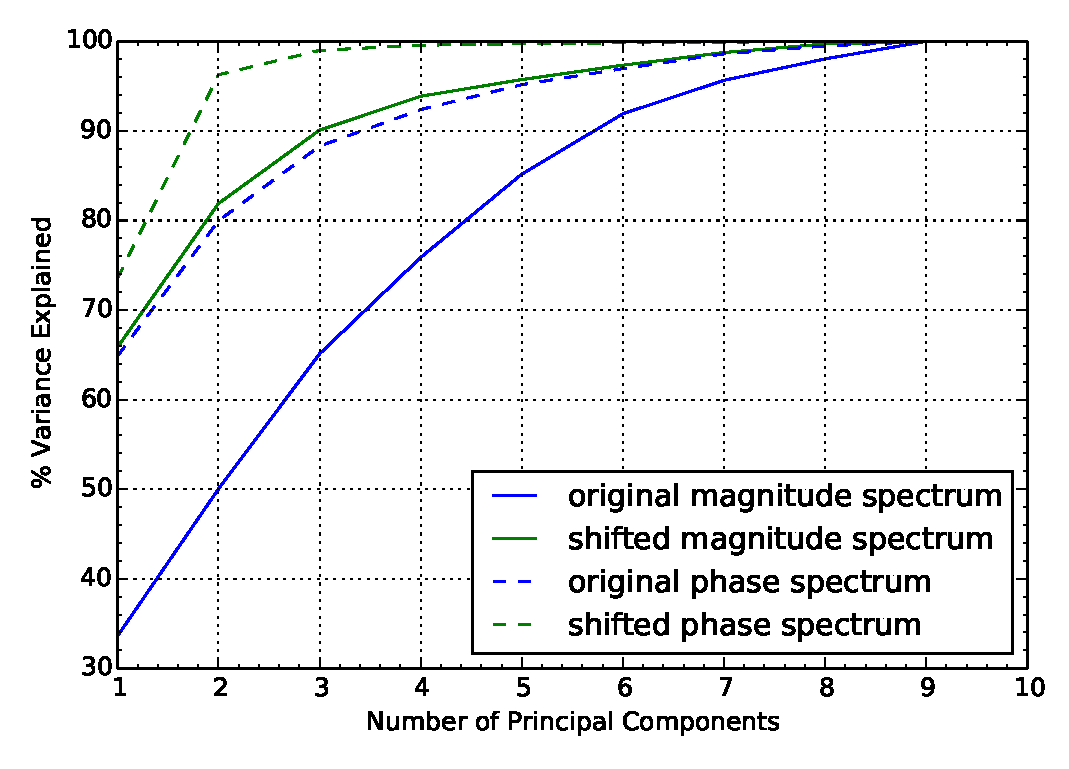
\includegraphics[width=0.5\linewidth]{eigenergy.pdf}
    \captionof{figure}{ Explained Variance.}
    \label{fig:eigenergy}
\end{center}%\vspace{1cm}

Figure~\ref{fig:eigenergy} compares the explained variance as a function of
number of principal components for the original and shifted spectra.  We require
about half as many principal components after applying our shifting procedure.
Much of the variance in the original catalogue arises from a feature, the
location of $f_{\rm peak}$, which is easily aligned.


\begin{minipage}{\columnwidth}
\makeatletter
\newcommand{\@captype}{figure}
\makeatother
\centering
\subfloat[Matches from PCA models using the original spectra]{%
  %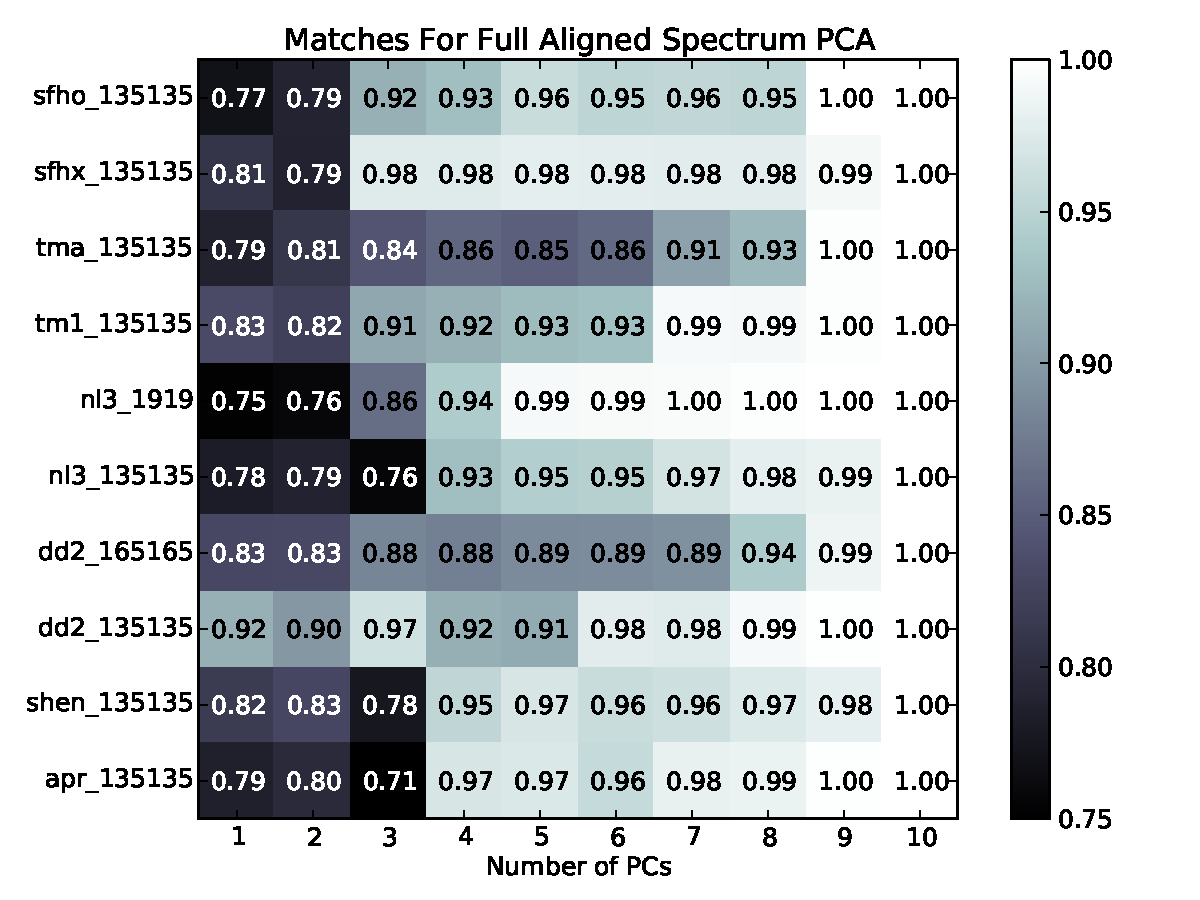
\includegraphics[width=0.45\linewidth]{shiftspec_ideal_matches.pdf}%
  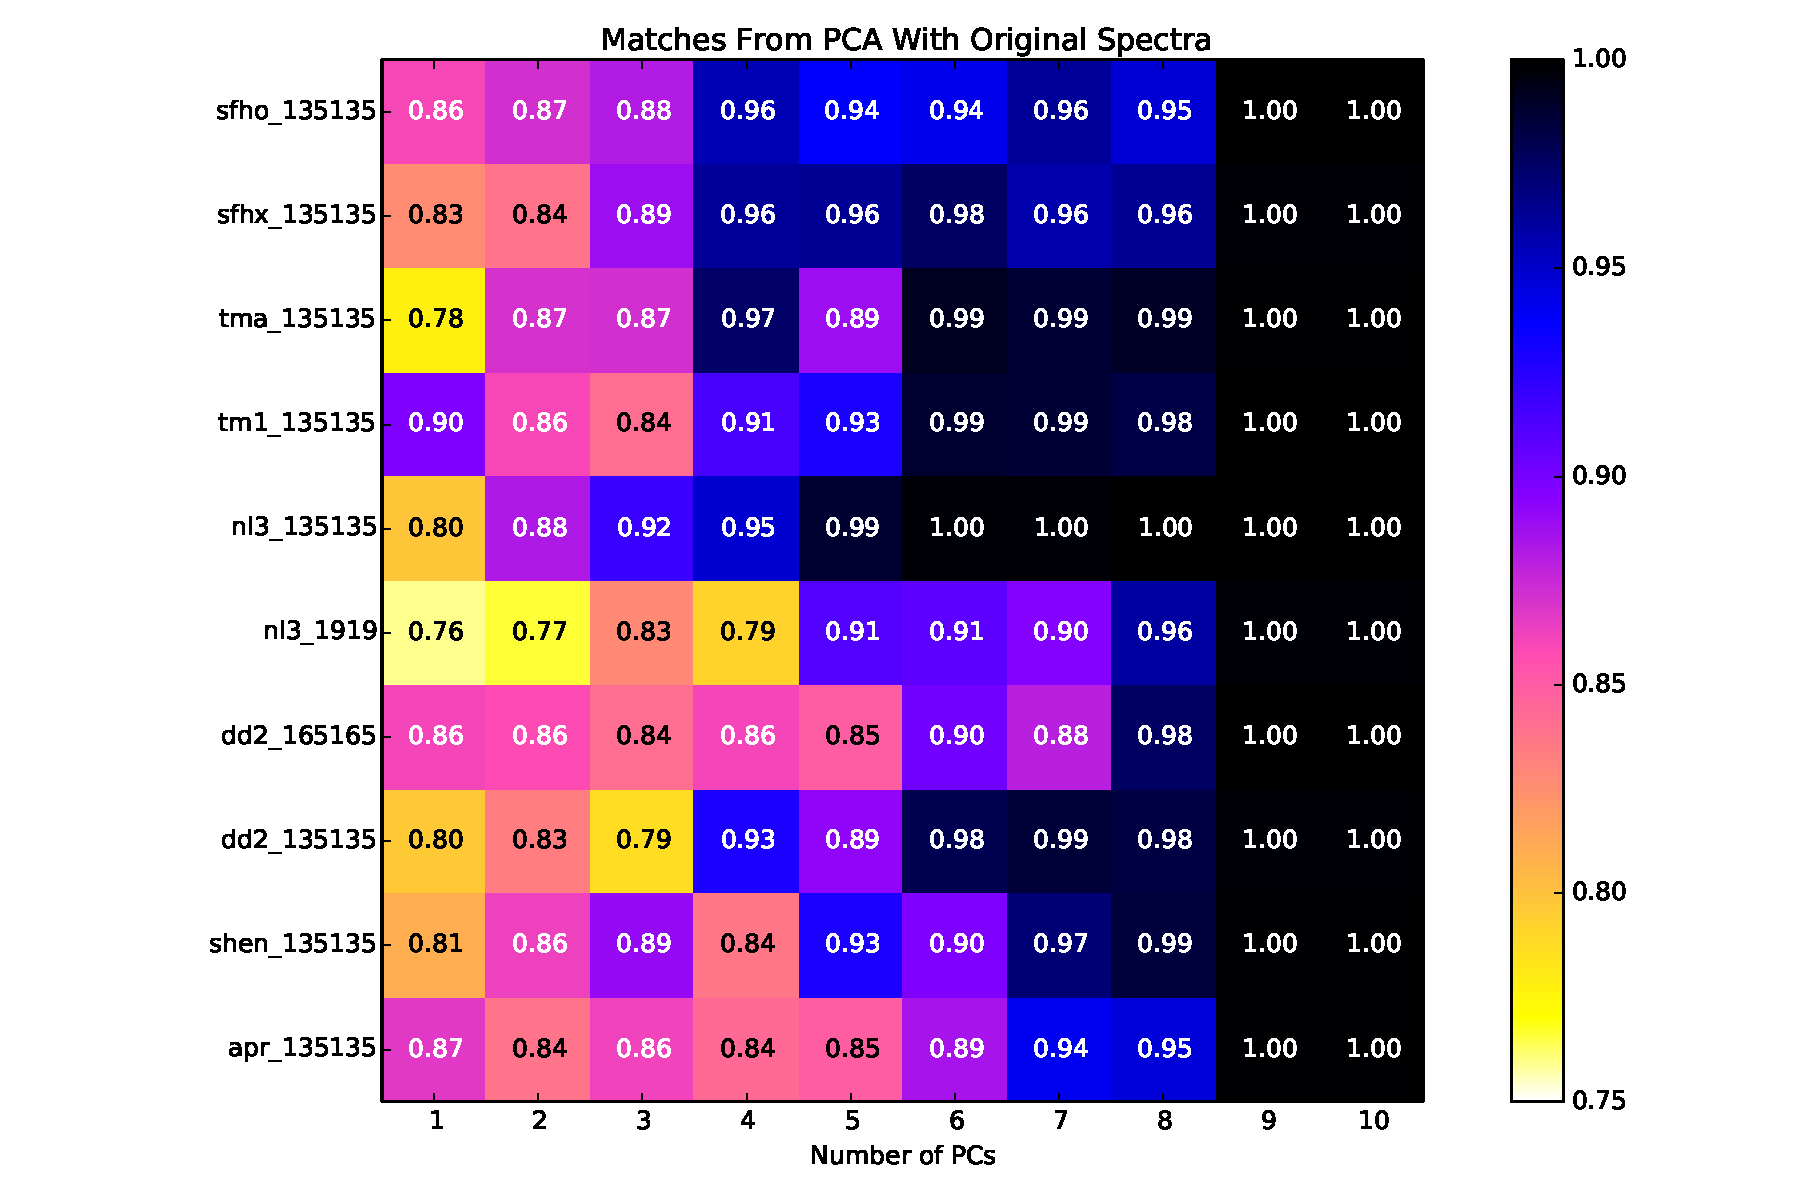
\includegraphics[width=0.45\linewidth]{fullspec_ideal_matches.pdf}%
  \label{fig:}%
}\qquad%
\subfloat[Matches from PCA models using the shifted spectra]{%
  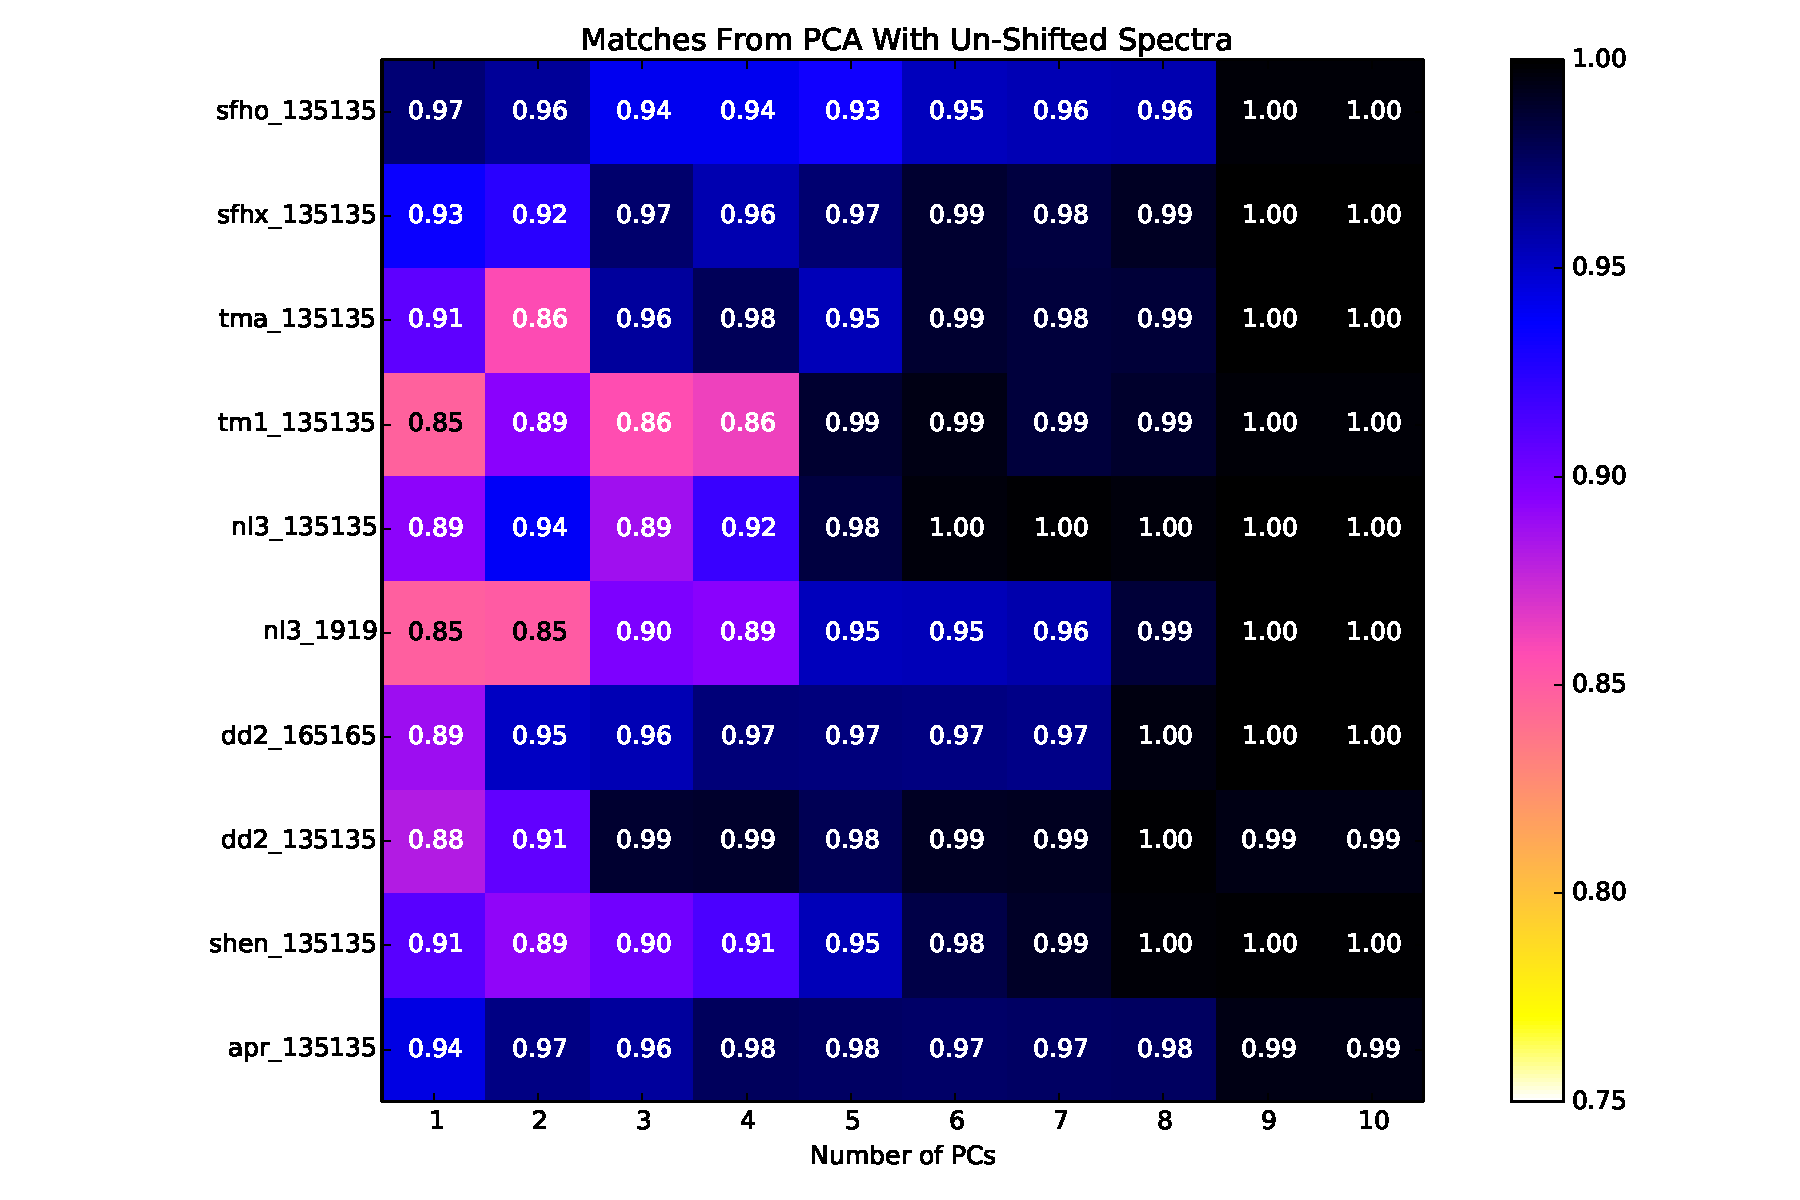
\includegraphics[width=0.45\linewidth]{unshiftspec_ideal_matches.pdf}%
  \label{fig:}%
}
\caption{Match as a function of number of basis functions used for all waveforms
in the catalogue (vertical axes).  Matches $\sim 90\%$ are achievable with even
a small number of components.}
\label{fig:matches}
\end{minipage}


Finally, figure~\ref{fig:matches} compares the matches for the waveforms in our
catalogue using the original and shifted spectra.  Provided we follow the
frequency shifting procedure outlined, we find that {\bf matches of
    $\mathbf{\sim 90\%}$ and above are easily realised using a small number of
    principal components}, far fewer than would be required using the un-shifted
data.

%----------------------------------------------------------------------------------------
%	CONCLUSIONS
%----------------------------------------------------------------------------------------

%\color{SaddleBrown} % SaddleBrown color for the conclusions to make them stand out

\section*{\centering Conclusions}

\begin{itemize}
\item Have demonstrated a method to construct a low-dimensional and reasonably
    accurate model using principal component analysis and a novel feature
    alignment scheme.
\item {\bf Some caveats}: small catalogue \& have only demonstrated ability to
    reconstruct \emph{training} data.
\item Applications include: burst parameter estimation follow-ups of BNS inspiral
    detections, Monte-Carlo simulations in un-modelled analysis
    and machine learning algorithms \& astrophysical interpretation waveform
    reconstructions from other burst algorithms.
\end{itemize}

%\color{DarkSlateGray} % Set the color back to DarkSlateGray for the rest of the content


 %----------------------------------------------------------------------------------------
%	REFERENCES
%----------------------------------------------------------------------------------------

%\nocite{*} % Print all references regardless of whether they were cited in the poster or not
\small{
\bibliographystyle{unsrt} % Plain referencing style
\bibliography{pmnspca_poster} % Use the example bibliography file sample.bib
}

%----------------------------------------------------------------------------------------
%	ACKNOWLEDGEMENTS
%----------------------------------------------------------------------------------------

%\section*{Acknowledgements}

%Etiam fermentum, arcu ut gravida fringilla, dolor arcu laoreet justo, ut imperdiet urna arcu a arcu. Donec nec ante a dui tempus consectetur. Cras nisi turpis, dapibus sit amet mattis sed, laoreet.

%----------------------------------------------------------------------------------------

\end{multicols}
\end{document}
